%%%%%%%%%%%%%%%%%%%%%%%%%%%%%%%%%%%%%%%%%
% Journal Article
% LaTeX Template
% Version 1.4 (15/5/16)
%
% This template has been downloaded from:
% http://www.LaTeXTemplates.com
%
% Original author:
% Frits Wenneker (http://www.howtotex.com) with extensive modifications by
% Vel (vel@LaTeXTemplates.com)
%
% License:
% CC BY-NC-SA 3.0 (http://creativecommons.org/licenses/by-nc-sa/3.0/)
%
%%%%%%%%%%%%%%%%%%%%%%%%%%%%%%%%%%%%%%%%%

%----------------------------------------------------------------------------------------
%	PACKAGES AND OTHER DOCUMENT CONFIGURATIONS
%----------------------------------------------------------------------------------------

\documentclass[twocolumn]{article}

\usepackage{blindtext} % Package to generate dummy text throughout this template 

\usepackage[sc]{mathpazo} % Use the Palatino font
\usepackage[T1]{fontenc} % Use 8-bit encoding that has 256 glyphs
\linespread{1.05} % Line spacing - Palatino needs more space between lines
\usepackage{microtype} % Slightly tweak font spacing for aesthetics


\usepackage[english]{babel} % Language hyphenation and typographical rules

\usepackage[hmarginratio=1:1,top=32mm,columnsep=20pt]{geometry} % Document margins
\usepackage[hang, small,labelfont=bf,up,textfont=it,up]{caption} % Custom captions under/above floats in tables or figures
\usepackage{booktabs} % Horizontal rules in tables

\usepackage{lettrine} % The lettrine is the first enlarged letter at the beginning of the text

\usepackage{enumitem} % Customized lists
\setlist[itemize]{noitemsep} % Make itemize lists more compact

\usepackage{abstract} % Allows abstract customization
\renewcommand{\abstractnamefont}{\normalfont\bfseries} % Set the "Abstract" text to bold
\renewcommand{\abstracttextfont}{\normalfont\small\itshape} % Set the abstract itself to small italic text

\usepackage{titlesec} % Allows customization of titles
\renewcommand\thesection{\Roman{section}} % Roman numerals for the sections
\renewcommand\thesubsection{\roman{subsection}} % roman numerals for subsections
\titleformat{\section}[block]{\large\scshape\centering}{\thesection.}{1em}{} % Change the look of the section titles
\titleformat{\subsection}[block]{\large}{\thesubsection.}{1em}{} % Change the look of the section titles

\usepackage{fancyhdr} % Headers and footers
\pagestyle{fancy} % All pages have headers and footers
\fancyhead{} % Blank out the default header
\fancyfoot{} % Blank out the default footer
\fancyhead[C]{Multi-Authority ABE for Bdrive$\bullet$ July 2018 $\bullet$ Vol. I, No. 1} % Custom header text
\fancyfoot[EL]{\thepage} % Custom footer text

\usepackage{titling} % Customizing the title section

\usepackage{hyperref} % For hyperlinks in the PDF
\usepackage{multicol}
\usepackage{graphicx}
\usepackage{caption}

  %
  \newcommand{\todo}[1]{
    \addcontentsline{tdo}{todo}{\protect{#1}}
    \marginpar{#1}
}

%----------------------------------------------------------------------------------------
%	TITLE SECTION
%----------------------------------------------------------------------------------------

\setlength{\droptitle}{-4\baselineskip} % Move the title up

\pretitle{\begin{center}\Huge\bfseries} % Article title formatting
\posttitle{\end{center}} % Article title closing formatting
\title{Multi-Authority Attribute Base Encyrption Scheme for Bdrive } % Article title
\author{%
\textsc{Marvin Petzolt}\thanks{TODO: fill} \\[1ex] % Your name
\normalsize TU Berlin \\ % Your institution
\normalsize \href{mailto:marvin.petzolt@protonmail.com}{marvin.petzolt@protonmail.com} % Your email address
%\and % Uncomment if 2 authors are required, duplicate these 4 lines if more
%\textsc{Jane Smith}\thanks{Corresponding author} \\[1ex] % Second author's name
%\normalsize University of Utah \\ % Second author's institution
%\normalsize \href{mailto:jane@smith.com}{jane@smith.com} % Second author's email address
}
\date{\today} % Leave empty to omit a date
\renewcommand{\maketitlehookd}{%
\begin{abstract}
\noindent TODO: Abstract % Dummy abstract text - replace \blindtext with your abstract text
\end{abstract}
}

%----------------------------------------------------------------------------------------

\begin{document}

% Print the title
\twocolumn[
    \maketitle
]


%----------------------------------------------------------------------------------------
%	ARTICLE CONTENTS
%----------------------------------------------------------------------------------------

\section{Introduction}

\lettrine[nindent=0em,lines=3]{B}
drive is a secure cloud storage where files get split up in smaller chunks that are saved speratly on different storage provider. To ensure end-to-end encryption a Bdrive client encrypts each of his chunks with the a one-time symmetric key that is then encrypted under his own public key. This encrypted key is called a file key and it is uploaded to the Bdrive server where it is stored securely. 

Since each device of the same user has a different private-public key pair, the client is in charge of making the file keys available for the new client. This is done by downloading each file key for the receptive file, downloading the public key of the new client, decrypting the file key with his own private key, encrypting it again with the public key of the new device and finally, uploading the new file key to the Bdrive server.

The number of file keys that need to be maintained raises with the number of clients. In addition Bdrive allows to share files between different users. The formula XXXX describes the number of file keys Bdrive need to store for each shared files between $u$ users, where each user $u_i$ has $d_i$ devices.

$$
n = \sum_{i \le u}{d_i} 
$$

Lets construct an example where the manager of a company wants to create a shared folder with all company employees. It is a medium sized company with 50 employees. At least haft of them have two Bdrive clients running. The manager wants to upload the 250 photos of the last company trip.
We end up by computing $3/2 * 50 * 250 = 18750$ file keys and for every new file uploaded 75 new file keys need to be uploaded. 

We reach the point where the classical public-key end-to-end encryption scheme does not scale anymore. 


\begin{figure*}[!ht]
\centering
    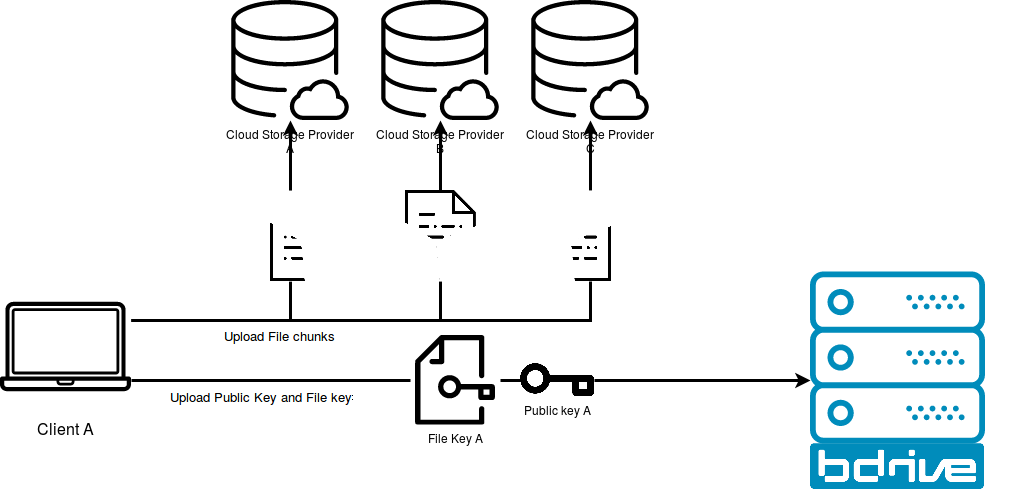
\includegraphics[width=0.7\linewidth]{img/bdrive1.png}\par 
    \caption{caption here}
\end{figure*}
\begin{figure*}[!ht]
\centering
    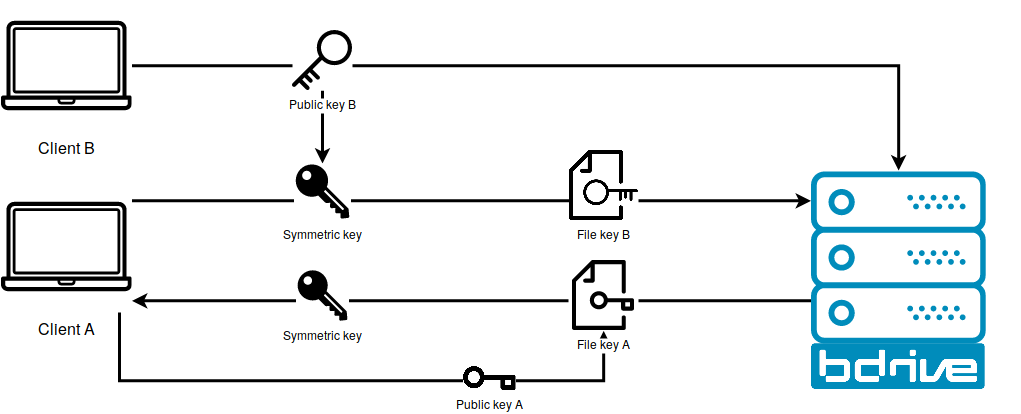
\includegraphics[width=0.7\linewidth]{img/bdrive2.png}\par
    \caption{caption here}
\end{figure*}


\section{Related Work}

Attribute Based Encryption (ABE), first introduced by Sahai and Waters \cite{sahai2005fuzzy}, is a cryptographic encryption scheme which encryptes under attributed that describe a user, rather than common known keys. This enables the encryptor to craft a cypher text over chosen attributes that can only be decrypted by any entity that holds a super set of matching attributes. Further, it is possible to embed the access policy in a tree inside the cipher text, where each node is contains \todo{fix encoding} “AND” or “OR” gates. If the attribute values are stored in the leafs, the decryptor can evaluate the tree in a post-order fashion and evaluate whether the root node yields “true” or “false”. This approach was first introduced by Bethencort, Sahai and Waters in Ciphertext-policy Attribute-Based Encryption (CP-ABE). \cite{bethencourt2007ciphertext}. 
It is also possible to do it the other way arround: Associate the user’s key with an access policy. Now, the encryptor needs only to encrypt the given plain text with the public key of specific attributes so that only user who hold the right keys are able to decrypt the cipher text. This approach is called Key-Policy Attribute Based Encryption (KP-ABE). \todo{cite} 
\todo{extend: Multi-ABE} 

%------------------------------------------------

\section{Security Requirements}
\label{sec:securityRequirements}
The core security requirements regarding Bdrive in the context of a multi-authority ABE scheme are the following:
\begin{itemize}
\item \textbf{Collusion resistance:} For two users it should not be possible to combine their attributes to archive a higher level 
\item \textbf{Inter-Company Sharing:} Since Bdrive would need to consider a multi-authority ABE scheme, it should not be possible for a company to decrypt or issue files of other companies if no explicit exception is given for certain files by a trusted company relationship. A companies attribute authority (AA) should be responsible for its domain. In the case of an inter company relationship, attributes needs to be issued across different companies. 
\item \textbf{Central Authority:} In a multi-authority setting usually a central authority is coordinating the different attribute authorities to identify users and prevent collusion. However, it should not be possible that the central authority has a global decryption power.  
\item \textbf{Secret Master key (if any):} Key recovery requires a secret and securely stored master key. It should solely function in the company domain and not globally. 
\item \textbf{Large Key Universe:} The key universe should be large so that Bdrive can act dynamically regarding attribution issuing and each company could define their own set of attributes. Further, a finite field of keys would restrict the number of possible users in the system, which is not intended.
\item \textbf{Adding new Attribute Authorities:} It should be possible to add new attribute authorities while runtime. Without either shutting down the system or recreating each key. 
\item \textbf{Key and Attribute revocation:} Either a period defining the lifetime of valid keys or a direct revocation mechanism ensures key and attribute revocation. In both cases the keys have a limited lifetime of two months. After this period the keys become invalid and have to be reissued.
Key attribute or whole key revocation should be possible to handle user management in terms of attribute promotion, attribute demotion and key revocation. Revoked keys are no longer able to decrypt the cypher text. 
\end{itemize}

On the other hand we are forced to loosen some security requirements that have hold in a RSA based environment. One Attribute Authority (AA) needs to issue the attributes for a group of users. This users are assigned to a designated company. Since the AA issues also the private keys for each attribute it holds also a master secret for this company domain and is in turn able to decrypt all users file of this company. While in the current cryptographic scheme enrolled in Bdrive an artificial master-key was implemented, it would still be possible to easily remove it from the system. This is not possible with the an ABE scheme. 


\section{Targets}
The target of this work will be to implement and define a multi-authority ABE scheme for Bdrive that fits the security requirements of the previous section. This approach will decrease the number of file keys stored on the Bdrive server dramatically and will make Bdrive scale better for a higher user workload. To evaluate this a prototype should be implemented that is able to up- and download files, to encrypt them symmetrically and encrypt the file key under a multi-authority ABE scheme. 

The minimal requirement is to implement a multi-authority ABE scheme where at least two AAs issue attributes to different users and the user are able to share a file between them. This file should only be encrypted using one file key. This implementation and system design summarized the security requirements of: Collusion resistance, inter-company Sharing, central authority, adding new authorities and Secret Master key. To implement and define this prototype Chase’s proposal of an multi-authority ABE scheme \cite{chase2007multi} in combination with the extension of Chase to deescalate the decryption power of the central authority \cite{chase2009improving} is used. 

The next step would be to implement the key-revocation, which is not trivial in an ABE setting. Optional is to extend the defined scheme with a large key universe. It is not clear yet whether this is even possible as it is proposed by Chase or if a complete different approach need to be taken to take this issue. 


%------------------------------------------------

\section{Concept}
The basic idea is, as proposed in \cite{chase2007multi}, to construct for each users a polynom of degree $d-1$, where $d$ donates the number of attributes in our system. 

To prevent collusion between user in a multi authority setting, the challange for each user needs to be individuell. But we still need to ensure that the encryption of message is indepenent of any user specific identifier, since the encryption progress should sourly depent on the attribute set known to the system.
To mitigate this problem a global identifier (GID) per users was introduced that is shown to each attribute authority (AA) to receive the corresponding private key for the users attributes. 
The central authority (CA) now has to make sure that the user dependent challange results in a global decryption key to decrypt the message.
In the fact that the CA has to be trusted since it computes the users private keys in such a way that on decyrption it reveals the global decryption key. 

In \cite{case2007multi} the CA generated random seeds that are distributed to the Attribute Authorities. Each authority uses this seed to deterministically create the users private key. Since the CA persesses the same seed and knows the users GID, it can also create the same private key and ensure that on decyrption the keys add up to reveal the global decyrption key.

We set the multi-authority scheme proposed by Chase 2007 as a baseline for the building block of the concept. It is defined in figure \ref{fig:chase-multi-auth}. $g^{y_{k,u}s}$ is the user depending blinded point of interesset, which is derivated from the pheudo random function $F(GID)$ with seed $s_k$. This seed is choosen by the CA in advance to ensure that the challanges for each authorities $k$ add up in $g^{y_0 - \sum^K_{k=0} y_{k,u}}$ to reveal the blinded master secret $g^{y_0 s}$, which is than used for decryption of the ciphertext. This step is nessecary to a) prevent collusion between users (so making the challange user dependent) and b) to make the encryption indepent of the user's GID (only use the systems public key). The authories should not know the secrets (seeds) of the other AAs so that it can not issue attributes without of its domain. So the CA needs to be trusted and honest since it generates the master secret ($g^{y_0}$) and distributes the secret seeds ($s_k$) and has global decryption power.  

\begin{figure*}[!h]
\begin{itemize}
	\item \textbf{System}:\\
	\textbf{Init}: Fix prime order groups $G$, $G_1$, bilinear map $e: G \rightarrow G_1$, and generator $g \in G$. Choose seeds $s_1, \dots, s_K$ for all authorities. Also choose $y_0 , \{t_{k,i}\}_{k=1...K,i=1\dots n} \leftarrow Z_q$. \\
	\textbf{System Public Key}: $Y_0 = e(g, g)^{y_0}$
	\item \textbf{Attribute Authority} $k$: \\
	\textbf{Auhtority Secret Key}: $s_k, t_{k, 1} \dots t_{k,n} $ \\
	\textbf{Authority Public Key}: $ T_{k, 1} \dots T_{k, n}$ where $T_{k, i} = g^{t_{k,i}} $\\
	\textbf{Secret Key for User } $u$: Let $y_{k,u} = F_{s_k}(GID)$. Choose random $d - 1$ degree polynomial $p$ with $p(0) = y_{k,u}$. Secret Key: $\{D_{k,i} = g^{p(i)/t_{k,i}} \}i \in A_u $.
	\item \textbf{Central Authority}:\\
	\textbf{Central Authority Secret Key}: $s_k$ for all authorities $k, y_0$.  \\
	\textbf{Secret Key for User} $u$: Let $y_{k,u} = F_{s_k}(GID)$ for all $k$. Secret Key: $D_{CA} = g^{y_0 - \sum^K_{k=0} y_{k,u}}$
	\item \textbf{Encryption for attributes set } $A_C$: \\
	Choose random $s \leftarrow Z_q$. $E = Y_0^s m$, $E_{CA} = g^s$, $\{E_{k,i} = T^s_{k,i}\}_{i \in A^k_C, \forall k}$
	\item \textbf{Decryption}:\\
	For each authority $k$, for $d$ attributes $i \in A^k_C \cap A_u$, compute $e(E_{k,i}, D_{k,i}) = e(g,g)^{p(i)s} = e(g,g)^{y_{k,u}s}$.  Interpolate to find $Y^s_{k,u} = e(g, g)^{p(0)s} = e(g,g)^{y_{k,u}s}$ for each authority $k$. Compute $Y^s_{CA} = e(E_{CA} , D_{CA})$. Combine these values to obtain $Y^s_{CA} * \prod^K_{k=1} Y^s_{k,u} = Y^s_0$. Then $m = E/Y_0^s$
\end{itemize}
\caption{Multi-Authority scheme as proposed by Chase 2007 in \cite{chase2007multi}. $A_u$ donates the attributes of user $u$. $A_C$ donates the attributes of the cipher text.}
\label{fig:chase-multi-auth}
\end{figure*}


However, as discussed in \ref{sec:securityRequirements} we want the company domain to remain sealed. That means that we don't want to have a global trusted authority that has global decyrption power. 
Chase addressed this issue in \cite{chase2009improving}, where she proposed the usage of an seeding network. Here every two AA's exchange seeds than combine them with the pheudorandom functions to produce the users private key. 

In the first step the master secret key $Y_0$ needs to be split apart the authorities. Each authority chooses independent a $y_k$ and sends $Y_k = e(g_1, g_2)^{y_k}$ to each other authority. Every authority than computes the global master public key $Y_0 = \prod Y_k = e(g_1, g_2)^{\sum y_k}$.

For every user the authority $k$ computes a random polynomial $p_k$ with the point of interest defined as $p_k(0) = y_k - \sum_{j \in \{1 \dots N\} \backslash \{k\}} R_{kj}$.

To build up our secret-seeding network, let $s_{kj}$ be the seed exchanged by authority $k$ with authority $j$ ($k \neq j$). For the user now to receive its decryption keys for authority $k$, he requests 
$Q_{kj} = g_1^{R_{kj}} * F_{s_{kj}}(GID)^{\delta_{kj}}$ for each authority $j, j \neq k$. $R_{kj}$ is choosen randomly by the authority $k$. The clue is to set $\delta_{kj}$ to either $-1$ if $j<k$ otherwise $1$. The user combines all collected $Q_{kj}$ decryption keys form each AA to compute his own unique, global decryption key $Q_u = \prod_{(j,k) \in \{1 \dots N\} \times (\{1 \dots N\} \backslash \{k\})} Q_{kj} = g_1^{\sum_{(j,k) \in \{1 \dots N\} \times (\{1 \dots N\} \backslash \{k\})} R_{kj}} = g_1^{R_u}$. Since all pheudo random functions are canceling out each other (depending on $\delta_{kj}$). Encryption happens in the same way as described in \ref{fig:chase-multi-auth}. 

The decryption part is also adapted in the way that each $p_k(0)$ that was found using interpolation, is multiplied together to that the user ends up with a global point of interest for this user. 

The full descritpion of this scheme and the adaption to the previous presented trused-CA setup is decribed in \ref{fig:chase-multi-auth-without-trusted-CA}.

We now successfully eliminated the trusted CA. However, several problems remain. How to add authorities? How to change attributes and revoke users from the system?

\todo{clarify $g_1$ stuff}
\begin{figure*}[!h]
\begin{itemize}
	\item \textbf{System}:\\
	\textbf{Init}: Fix prime order groups $G$, $G_1$, bilinear map $e: G \rightarrow G_1$, and generator $g \in G$.

	\item \textbf{Attribute Authority} $k$: \\
	\textbf{Auhtority Secret Key}: $y_k \leftarrow Z_q$ (only used once), $s_{kj} = s_{jk}$ as exchanged with each authority $(k,j) \in (\{1 \dots N\} \backslash \{k\}), t_{k, i} \leftarrow Z_q \forall i \in A_k$ \\
	\textbf{Authority Public Key}: $Y_k = e(g,g)^{y_k}$, $ T_{k, 1} \dots T_{k, n}$ where $T_{k, i} = g^{t_{k,i}} $\\
	\textbf{System Public Key}: Each authority computes $Y_0 = \prod Y_k = e(g, g)^{\sum y_k}$\\
	\textbf{Secret Key for User } $u$: For $j \in \{1 \dots N\}\backslash \{k\}$: 
	$Q_{kj} = g_1^{R_{kj}} * F_{s_{kj}}(GID)^{\delta_{kj}}$, $R_{kj} \leftarrow Z_q$ and set $\delta_{kj}$ to either $-1$ if $j<k$ otherwise $1$.

	Choose random $d - 1$ degree polynomial $p$ with $p_k(0) = y_k - \sum_{j \in \{1 \dots N\} \backslash \{k\}} R_{kj}$. 

	Secret Key: $\{D_{k,i} = g^{p(i)/t_{k,i}} \}i \in A_u $.

	User computes: $Q_u = \prod_{(j,k) \in \{1 \dots N\} \times (\{1 \dots N\} \backslash \{k\})} Q_{kj} = g_1^{\sum_{(j,k) \in \{1 \dots N\} \times (\{1 \dots N\} \backslash \{k\})} R_{kj}} = g_1^{R_u}$

	\item \textbf{Central Authority}:\\
	Issues unique $GID$ for user $u$.
	\item \textbf{Encryption for attributes set } $A_C$: \\
	Choose random $s \leftarrow Z_q$. $E = Y_0^s m$, $E_{1} = g^s$, $\{E_{k,i} = T^s_{k,i}\}_{i \in A^k_C, \forall k}$
	\item \textbf{Decryption}:\\
	For each authority $k$, for $d$ attributes $i \in A^k_C \cap A_u$, compute $e(E_{k,i}, D_{k,i}) = e(g,g)^{p(i)_{k}s}$.  Interpolate to find $P_k = e(g, g)^{p(0)_{k}s} = e(g,g)^{s(y_k - \sum_{j \neq k} R_{kj})}$. Multiply $P_k$ together to get $V = e(g,g)^{s(\sum\{y_k\} -R_u)} = Y_0^s / e(g^{R_u}, g^{s})$. Compute $e(Q_u, E_1) * V = e(g^{R_u}, g^s) * V = Y_0^s$. Recover $m$ by $E/ Y_0^s$.
\end{itemize}
\caption{Multi-Authority scheme as proposed by Chase 2007 in \cite{chase2007multi}. $A_u$ donates the attributes of user $u$. $A_C$ donates the attributes of the cipher text.}
\label{fig:chase-multi-auth-without-trusted-CA}
\end{figure*}


%------------------------------------------------

\section{Method of Evalution}

%----------------------------------------------------------------------------------------
%	REFERENCE LIST
%----------------------------------------------------------------------------------------

\bibliography{multi-authority-abe-proposal} 
\bibliographystyle{ieeetr}

%----------------------------------------------------------------------------------------

\end{document}
